\documentclass[12pt, oneside]{amsart}
\usepackage[margin=1in]{geometry}                % See geometry.pdf to learn the layout options. There are lots.
\geometry{letterpaper}                   % ... or a4paper or a5paper or ... 
\usepackage[parfill]{parskip}        % Begin paragraphs with an empty line rather than an indent
\usepackage{graphicx}
\usepackage{amssymb}
\usepackage{epstopdf}
\usepackage{url}
\usepackage[comma,authoryear]{natbib}
\DeclareGraphicsRule{.tif}{png}{.png}{`convert #1 `dirname #1`/`basename #1 .tif`.png}

% Different font in captions
\newcommand{\captionfonts}{\small}

\makeatletter  % Allow the use of @ in command names
\long\def\@makecaption#1#2{%
  \vskip\abovecaptionskip
  \sbox\@tempboxa{{\captionfonts #1: #2}}%
  \ifdim \wd\@tempboxa >\hsize
    {\captionfonts #1: #2\par}
  \else
    \hbox to\hsize{\hfil\box\@tempboxa\hfil}%
  \fi
  \vskip\belowcaptionskip}
\makeatother   % Cancel the effect of \makeatletter

% My contribution is:  What am I doing, how is it unique, what are the steps.

\title{An Open Model for Climate Behaviors}
\author{James Rising}

\begin{document}
\maketitle

\begin{abstract}
A system dynamics model of the behaviors that produce climate change can facilitate effective policy-making by helping to identify leverage points.  This project aims to construct a model of the social system surrounding driving behaviors, while developing an open, extensive framework applicable to a wide variety of social issues.  New structures for system modeling and analysis are needed to support this model, and are founded in self-organized criticality and the tools of network theory.
\end{abstract}

\section{Introduction}

Anthropomorphic climate change and environmental degradation are among the most pressing issues of our time, and while an impressive array of new green technologies and strategies have arisen in recent years, the human behaviors that drive climate change remain intractable.  Within the United States, carbon tax and cap and trade legislation has stalled; environmentally damaging farm practices continue to be the norm; industry and agricultural subsides obscure the costs of business; and consumers continue to favor heavily processed, packaged, wasteful, and polluting products.

These problems stem from motivations deeply embedded in our society, economy, and government.  Moreover, they are mutually reinforcing.  Politicians are unwilling to advocate policy changes they fear would be unpopular; companies are hesitant to take climate change action on their own; and efforts on the part of consumers to avoid environmentally damaging purchases are difficult without the support of business and government.  If the U.S. raises its environmental standards, it can ultimately encourage more imports from countries with lower standards.  If research helps make a green technology economically attractive by saving businesses money, the total effect may rebound as businesses use the money saved to invest in dirtier industries \citep{greening2000energy}.  \cite{Forrester1991} notes that ``the very nature of the dynamic feed-back structure of a social system tends to mislead people into taking ineffective and even counterproductive action.''

It is these counterintuitive, systemic, and cybernetic effects that motivate the approach for this project.  All complicated systems consist of interwoven feedback loops, often held in an overdetermined homeostasis.  That equilibrium is characterized by both minimizing feedback loops, and maximizing ones.  While the effects of some actions, whether they are new laws, citizen movements, or business decisions, are minimized and effectively dismissed, other changes will be reinforced and amplified.  These ``leverage points'' are places where small changes can make pervasive differences.  Due to the structural nature of all systems, from ecosystems to economies, leverage points are common, if difficult to identify \citep{meadows1997places}.  In addition, the persistent pressures of the market may place society in a ``critical state'' \citep{lux1998scaling}, where small shifts can avalanche \citep{frette1996avalanche}.

The behaviors that cause climate change, including the use of outdated energy-generation technology, wasteful agricultural practices, and unsustainable transportation habits, are mutually reinforced by our entire economic, cultural, and political systems.  The goal of this project is to identify the leverage points in the social system surrounding U.S. behaviors that promote climate change and environmental damage.  A high-dimensional numerical model will be used to represent these behaviors, based on the techniques of system dynamics.  In developing this model, there are new opportunities to advance the field of human system modeling, using contributions from network theory.

The coupling of human and natural systems results in new layers of complexity, which have only recently begun to be explored \citep{liu2007complexity}.  These include feedback, non-linearity, resilience, and spacial heterogeneity.  This emerging research could benefit from a new modeling framework which can apply the temporal sophistication of system dynamics to the spacial heterogeneity typical of coupled systems.

The strengths of Columbia's PhD in Sustainable Development support this work, with the rigor of its economic foundations, the strong foundation it provides in the natural and human sciences, and the many opportunities provided under the Earth Institute and the Center for Research on Environmental Decisions (CRED) Lab.  Material from this project will form the basis for the author's dissertation on the opportunities for society to adapt to the new demands of a climate-strained world.  With the aid of the EPA's support and feedback, this unique framework has the potential to dramatically improve our capacity to model large, heterogenous systems and to understand the complex roles of existing institutions in influencing our climate behaviors.

\section{Behavior and Modeling Literature}

A wide range of models have been developed to understand pro-environmental behavior and try to discover how to motivate it.  Early models presumed that pro-environmental behavior was motivated by common-sense factors, such as information, rationality, community orientation, values, and the satisfaction of needs, but these had mixed results \citep{kollmuss2002mind}.  \citet{Hines1986} did a meta-analysis of 128 models and found evidence for the roles of knowledge of the issues, knowledge of action strategies, locus of control, attitudes, verbal commitment, and an individual sense of responsibility.

The models discussed by \citeauthor{kollmuss2002mind} and \citeauthor{Hines1986} represent an `agency' approach to explaining individual behaviors, and have limited applicability to studying society-wide dynamics.  \citet{redclift1994social} note,
\begin{quotation}
\begin{small}
The great majority of individuals may be `locked into' patterns of daily activity (such as private car use) which they know to be environmentally destructive.  Only if the spatial separations of work, shopping, leisure and residence were changed, or if public investment into socialized transport provision were greatly increased and transformed would individuals have a meaningful \emph{choice} to make about transport options for themselves.
\end{small}
\end{quotation}

A number of social approaches are emerging for encouraging pro-environmental behavior within groups, including deliberative and inclusionary processes or procedures (DIPS) and community social marketing for sustainability \citep{bloomfield1998deliberative, mckenzie1999fostering}.  While these developments are exciting, their methods will not be deeply engaged in this project.  DIPS has shown the powerful role that can be played by round tables and citizen juries, which should be included in any search for leverage points.  Social marketing groups are one likely beneficiary of the results of this project.  A large literature exists concerning the effectiveness of social change initiatives under community psychology.  \citep{Hirsch2007} argues that the models used by community psychologists are typically unidirectional, and proposes the use of system dynamics to enrich them.

The foundational work in system dynamics includes Ludvig von Bertalanffy's formative models of natural systems \citeyearpar{von1973general}, Jay Forrester's work in organizational dynamics \citeyearpar{forrester1961industrial}, and Donella Meadows's \emph{Limits to Growth} \citeyearpar{meadows2004limits}.  The techniques of system dynamics have been applied to many fields relevant to this project, including urban growth and decline \citep{alfeld1976introduction, forrester1971urban}, energy policy \citep{Naill1992}, environment management \citep{fletcher1998use, Guo2001}, public health \citep{Homer2001}, and social change initiatives \citep{repenning2002simulation}.\footnote{For an introduction to the tools and methodologies of system dynamics, see \cite{sterman2000business} for model-making,  \cite{senge2006fifth} for intuition, and \cite{meadows1997places} for leverage points.}

In recent decades, system dynamics has evolved a focus on small models, for the purposes of education and the development of mental models \cite[see][]{senge2006fifth, sterman1985strategem}.  Even in the large System Dynamics National Model, several economic sectors were collapsed into two, capital plant and consumer goods, for the purpose of clarity \citep{Forrester1991}.  This project represents a departure from that literature: while system models have an important role to play in education, the granularity necessary for identifying small leverage points requires a model that will not be conducive to attempts to understand it in full.  In addition to peer review of subsections, a variety of techniques exist to validate system dynamical models, many of 
which are readily adaptable to a computation framework \citep{barlas1996formal}.

\cite{ahmad2004spatial} integrates geographic information system modeling (GIS) and system dynamics into a new modeling approach called spacial system dynamics (see figure \ref{fig:ssdarch}).  The technique of combining the temporal modeling power of system dynamics with geographic data has been used for flood management \citep{ahmad2006intelligent}, water resource modeling \citep{vivoni2009semiarid, roach2009compartmental}, and invasive species spread \citep{bendor2006spatial}.  In spacial system dynamics, GIS provides the parameters by which the system models operate.  This project extends that integration, using a powerful network-based approach.
\begin{figure}[htb]
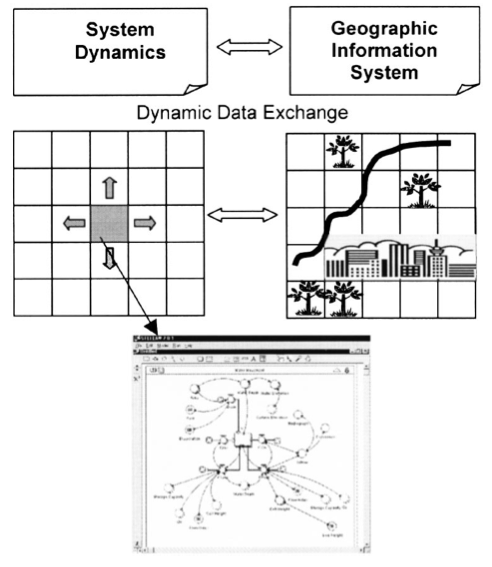
\includegraphics[width=3.5in]{ssdarch.png}
\caption{Architecture of the spacial system dynamics approach, reproduced from \cite{ahmad2004spatial}.  System dynamics handles temporal modeling, which the parameters of each cell are determined by GIS.}
\label{fig:ssdarch}
\end{figure}

\section{Methods}

The U.S. accounts for 20\% of carbon dioxide emissions, and almost four times the per-capita emissions of China.  The international production of imported goods for American consumers is responsible for additional greenhouse gasses, deforestation, resource extraction, and waste.  While global warming and climate change are by no means a problem solely of the developed world, we represent a disproportionate impact, and have a corresponding share of the responsibility.  This project focuses on the American consumer, through the policies, businesses, imports, environment, and political economy surrounding and influencing their actions.

Of the many fields used to model the factors that influence our habits, from psychology to economics, system dynamics provides a number of advantages exploited by this work.  System dynamics explicitly (and visually) describes feedback loops and policy conditions, which helps researchers describe relationships, experiment with policy changes, and illustrate the results.  System dynamics provides quantitative results, which can be verified, as well as established small-model behaviors.  Finally, existing models, such as the World3/2000 model used by \citeauthor{meadows2004limits} and Forrester's urban dynamics model, are available as a baseline.

In this project, environmental behavior is broadly defined as any institution which affects the status of environment variables.  If the use of coal power plants declines, it is taken to be a societal behavior, influenced by a variety of factors.  The decision-making process, as describe in agency models, is excluded from the model for several reasons.  First, decision-making is complicated and personal, and the principles of individual decision-making cannot be safely applied to an aggregated population \citep{may1954intransitivity}.  Second, causality within a system is poorly defined, where ``effects'' often influence their causes.  Third, we are interested in the pragmatic influences and results of these decisions, not the decision-making process itself.

One weakness of system dynamics is that it is hugely aggregative.  In traditional system models, distinguishing even between demographic segments (say, children and adults) requires reproducing all of the relevant relations influencing them both, as well the dynamics between them.  In addition, system models handle space poorly, tending to treat a distributed stock, such as arable land, as a single lump sum.

This project resolves these aggregation issues by using networks, similar to the spacial system dynamics framework.  The world of social interaction is a networked and a spatial world, where different rules apply to different regions.  Without this added complexity, the model would be unable to function on a sufficiently fine-grain to identify the particular institutions at the heart of climate change leverage points.  Rather than applying a single model to a system distributed in space, each region (represented as a node in a network) contains its own model, and these models are interconnected along the network.

The use of networks help capture two additional features of the social system: self-similarity and self-organized criticality.  In human systems, many of the same principles are exhibited at many different scales: globally, nationally, within an metropolitan region, and within a single institution \citep{song2005self}.  For example, a state's average pollution depends on the pollution in each of its counties, and the same dynamics apply to both scales.  Within climate prediction research, the process of moving between resolution scales is called downscaling, and the literature on both dynamical and statistical downscaling can inform this process \citep{murphy1999evaluation}.

This highlights the complementary role of time series data in this project.  In traditional system models, time series values are only used for parameter tuning and model verification.  The endogenous dynamics of a system determine its complete behavior, so there is little role for external data \citep{Forrester1991}.  In this framework, data drives both the downscaling process and helps define the pattern of heterogeneity between regions.

Self-similarity is one characteristic of self-organized critical (SOC) systems.  Society is rife with SOC systems, and examples have been studied in finance, disasters, and social networks \citep{turcotte2002self}.  Typical of SOC systems, many social systems exhibit the small-world property \citep{watts1998collective}, scale-free behavior \citep{barabasi1999emergence}, and hierarchical modularity \citep{ravasz2002hierarchical}.  Each of these is integrated elegantly into the proposed system, using multiple networks to represent different resolution scales.  This project takes advantage of self-similarity to identify smaller leverage points, and to do so extends the scope of spacial system dynamics to handle a hierarchical sense of space.

One more contribution from computer science is used in this project: an open interface for contributions.  In describing a large number of the factors that influence climate changing behaviors, and identifying small leverage points, this model benefits from having a large size.  By creating a way for other researchers to contribute to it, along with providing analysis of those contributions to help in their evaluation and review, the project becomes both more manageable and more useful.  As a platform for researches to run their partial models within a larger context, this framework can help to identify both strengths and contradictions between existing models of parts of society.

Unlike climate models, the purpose of this behavioral model is not to predict future states, but to capture the dynamics implicit in institutional relationships.  By developing computational tools for analyzing the model and running experiments, the high-dimensional model can be analyzed to identify key elements, relationships, and loops which can significantly effect the dynamics of the whole system.  Following  \cite{meadows1997places}, the system will consider the following potential points of leverage: changes in parameters, buffer sizes and flow speeds, the strength of feedback loops, and the structure of information flows.

Ten fundamental components are necessary to support an open, self-similar, networked system dynamics model, as described.  Each component represents a variety of prior work, but their combination is one this project's significant contributions.

\begin{description}
\item[A Framework of Partial Models] The full project consists of a framework and partial models.  The aspects described here are properly aspects of the framework, which forms the basis upon which relationships can be described and modeled.  The partial models, each of which applies to a particular region or collection of network nodes, overlap, interact, and reinforce each other.  Below, the terms ``framework'' and ``partial models'' are used to distinguish these aspects.
\begin{figure}[htb]
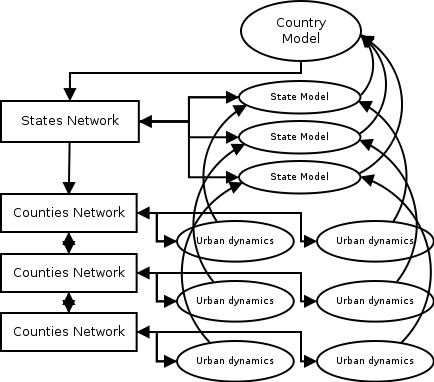
\includegraphics[width=4in]{architecture.png}
\caption{Partial architecture of the full model.  Aggregate dynamics from the Country Model are distributed through the States Network to each state's model (which is a modified version of the Country Model).  The State Models relay stocks between each other through the States Network, and inform the Country Model.  Each node in the State Network is associated with a Counties Network (that is, each state is divided into counties), with edges connecting the networks.  The results of each State Model are further distributed to Urban dynamics models, by way of the Counties Networks, and these dynamics further refine the State Models' dynamics.}
\end{figure}

\item[Conditional Self-Similarity] A partial model can describe the behaviors of both aggregate variables as well as apply to subregions.  Rather than explicitly duplicating the partial models to each levels of specificity, the framework applies a kind of fractal analysis, where global dynamics are modeled with global parameters, but with the potential to ``drill down'' to arbitrary levels of detail, reproducing the self-similar behaviors (see figure \ref{fig:selfsimodel}).  At each scale, the dynamics can be modified to reflect that sub-region more accurately.  This approach is grounded in complex systems theory \citep{morel1999through}.
\begin{figure}[htb]
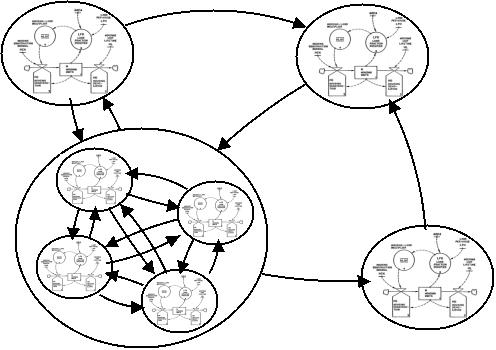
\includegraphics[width=4.5in]{selfsimodel.jpeg}
\caption{Self-similarity in system dynamics.  Each region is represented as a node, and each node may be associated with a further division of the region with another network.}
\label{fig:selfsimodel}
\end{figure}

\item[Multiple Network Maps] Different dynamics work upon different networks.  For example, the United States can be modeled for climate change by placing it on a grid, but people travel on roads, where the effective distance between two points is determined by the properties of the roads between them.  Information and culture flow in ways that are even more removed from the physical landscape.  The framework supports the use of multiple maps, both to represent different scales (e.g. state vs. county maps) and the different ways stocks flow between nodes (e.g. across land or along roads).  Demographics and corporate relations can also be encoded as networks, easing the need to reproduce dynamics across the different groups.\footnote{The author has analyzed Internal Revenue Service migration data and airline flight prices to form potential networks.}

\item[Monte Carlo Experiments with Stochastic Allotments] Sub-region dynamics can depend significantly on what portion of the aggregate allotment of each variable they represent.  The problem of determining the relevant parameters is not well-constrained.  Rather, Monte Carlo experiments over a range of initial conditions can be used to produce spread of results \citep{liu1998sequential}, and these compared to real data (see \ref{fig:trialestimate}).
\begin{figure}[htb]
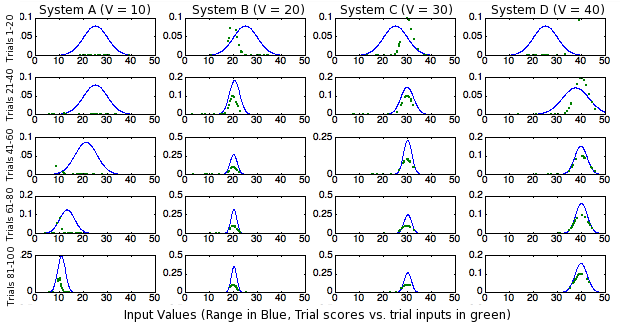
\includegraphics[width=6in]{trialestimate.png}
\caption{Example of a trial-based approach to dividing an aggregate stock.  Four simple systems (A-D) are modeled, which combine to represent a total stock of 100 units.  The actual division of that stock is for A = 10 units, B = 20, C = 30, and D = 40.  However, this information is not provided to the estimation system, which only has access to result values, which it uses to score 'trial' divisions.  Over the course of 100 trials, the values for B and C are quickly determined, and A and D are approached as well.}
\label{fig:trialestimate}
\end{figure}

\item[Associated Time Series Data] Every system component can be associated with a collection of time series data, with associated confidence values.  This data can be used for verifying the model, tuning parameters, scoring the results of a Monte Carlo run, or providing a fictional pressure representing missing relationships, along lines inspired by simulated annealing algorithms \citep{corana1987minimizing}.  In addition, each variable and data series will have a strict units definition to ensure consistency across the data and partial models.

\item[Open Exploration and Contributions] The framework will have an interface on the Internet, where people can explore its predictions, experiment with its parameters, and upload partial models as proposed additions.  The framework will use the libraries in FreeMat, an open source implementation of the MATLAB language, to make both data and model contributions relatively easy.  Eventually, a visual interface, as in the STELLA or Vensim software tools, can be added.  Group model building is widely used in system dynamics both for education and as a tool for creating accurate models \citep{rouwette2002group}.

\item[Meta-Model Evaluation of Contributions] One of the purposes of the framework is to inspect the behavior of partial models to determine how well they match historical data and other predictions.  \citet{barlas1996formal} describes a variety of techniques for validating models, some of which are readily adaptable to an programatic computation.

\item[Meta-Model Identification of Leverage Points] The framework will be able to intelligently seek-out and propose leverage points.  A combination of random experiments and hill-climbing algorithms can be used to identify these points.  The system parameter estimation methods in \citet{graham1976parameter} can also be used, by applying the model to idealized data sets.

\item[Memetic Transfer of Partial Models] The partial models describe both societal habits and policies, which have the potential to change and spread \citep{pech2004memetic}.  Indeed, this propagation of new ideas will play a large role in ultimately changing our climate change behaviors.  Therefore, the regions of applicability for partial models should be able to change, and other partial models can mediate this memetic transfer.

\item[Integration with Climate Models] Actual changes in climate will have a strong effect on behavior, so climate prediction must inform the model as a whole.  Initially, the framework can use pre-computed results from climate models, but climate change represents a coupled natural and human system, so ideally the integration would be deeper.  Incorporating a general climate model (GCM) into this framework presents a considerable computation challenge, but few conceptual difficulties.  The three-dimensional climate grid of a GCM can be incorporated as another network map, and the dynamics in each GCM cell are analogous to the framework's partial models.  The Community Earth System Model (CESM), described by \citet{blackmon2003towards}, is a reasonable choice for this.
\end{description}

\section{Next Steps}
\label{sec:implementing}

The process for proceeding with this project follows four overlapping phases: additional research, framework implementation, model development, and analysis.

The outstanding research questions include the following:
\begin{itemize}
  \item What mathematical procedures best address the dual constraints of downsampling and time-series data, to inform system parameters?  The sub-regions for downscaling may redistribute aggregate stocks between them (along their connecting edges), but must remain true in aggregate and approximate relevant time series data.
  \item How to ensure that incomplete models do not distort dynamics?  The model will evolve over time as more institutions are added.  When a relevant institution is missing, but its effects are reflected in the data, the model must ``fail gracefully,'' either by distorting results only locally, or by inferring the existence of unrepresented variables if the existing dynamics cannot account for them.
  \item How best can the model be visualized?  Systems that describe different regions are often related, and share components in ways that is difficult to represent.  Formalizing the theoretical concepts of a multi-level network, a multi-network system, and a multi-system component will inform this.
\end{itemize}

To give a sense of the timeline for this project, the framework implementation can occur in the following steps:
\begin{enumerate}
  \item A minimal framework, developed in MATLAB, is needed that can combine both time-series data and system dynamical relations, and reproduce the dynamics of other authors reliably.  At this point, relationships from the baseline model (e.g., World3/2000) can be reproduced and checked.
  \item A language for describing multi-level networks and self-similar system models will be developed in MATLAB, and incorporated into the dynamics framework.  Incorporating these pieces requires tools from climate model downsampling and Monte Carlo experiments.
  \item The self-similar system is formalized and implemented within an object oriented framework.  The MATLAB models are then incorporated using the open source FreeMat library.
  \item Basic evaluation techniques are added, to ensure that partial models reflect the dynamics observed in data, and for tuning the parameters that knit together distinct partial models.
  \item A website with documentation and a system for contributing to the model is built, as well as a way for researches to peer-review and expand each other's models.
  \item Analytics are developed for finding leverage points: first to identify driving loops, then to suggest key parameters, and finally to propose structural adjustments.  Both these techniques and the ways they present their results will need to evolve as they produce more results.
  \item Extensions of the model framework, such as memetic transfer and climate coupling, can be explored.
\end{enumerate}

The first four steps, constituting the fundamental framework, require approximately a year of research, implementation, and evaluation (concurrent with Columbia's PhD curriculum).  The second year of this project is devoted to developing the model systems and networks and improving the leverage point analysis.

It is difficult to estimate the number of system elements necessary to best support the search for leverage points.  Nation-wide models range in side considerably, from 283 variables (stocks, equations, parameters, and outputs) for World3/2000 to over 2000 in the System Dynamics National Model.  The range of relevant institutions is even larger-- the federal government has approximately 495 agencies\footnote{Based on a count of the ``A-Z Index of U.S. Government Departments and Agencies: Alphabetical list of organizations in the federal executive, legislative and judicial branches'' available at \url{http://www.usa.gov/Agencies/Federal/All_Agencies/Includes/Agency_Index.pdf}}, while the number of international NGOs and GOs is around 35,000\footnote{The Yearbook of International Organizations lists 34,995 international NGOs and IGOs}.  The monumental \emph{Encyclopedia of World Problems and Human Potential} has identified 56,135 ``problems,'' ranging from \emph{Loss of cultural diversity} to \emph{Youth gangs}, and identified within them 2,675 environmental feedback loops, ``problems that are implicated in many negative feedback systems concerning the natural environment''.\footnote{From \url{http://www.un-intelligible.org/projects/loops/looplynx.php\#stat}}  If each of those were properly modeled, they represent thousands of opportunities to break the cycle of environmental destruction.

The framework also allows for a large number of experiments, with different variables for measuring the effectiveness of possible leverage points.  Different researchers may place different emphasis on the production of $CO_2$ and other chemicals, the wealth or well-being of populations, and the health and diversity of ecosystems.\footnote{For example, the following expression combines the Human Development Index and the Living Planet Index (both estimated at the current time) to capture the needs of current and future generations:
\[
S_{SD} = \int_{t=t_{now}}^{t_{end}} I_{HD}(t) I_{LP}(t) e^{t/\tau} dt + e^{-t_{end}/\tau} \left(\tau^2 \frac{d I_{HD} I_{LP}}{dt}(t_{end}) + \tau I_{HD}(t_{end}) I_{LP}(t_{end})\right)
\]
where $I_{HD}$ and $I_{LP}$ are the Human Development Index and the Living Planet Index \citep{loh2005living}, respectively, based on OLS models; $t_{end}$ is the end time of the simulation; the time constant $\tau$ represents declining confidence in the model's results, and the second term uses the ending slope to extrapolate as $t \to \infty$.}

\section{Conclusion}

The complexity of the social, political, and economic system surrounding climate change requires new tools, drawing from the strengths of many fields.  The modeling framework described represents not just than an expansion or knitting together of existing models, but a new construct which elegantly draws on the strengths of these different techniques.  By combining system dynamics, networks, self-similarity, time series data, and computational analysis, this framework can capture the dynamics of social systems on a finer scale than previously possible.

This research has a considerable potential to inform policy decisions concerning the difficult problems of climate change and environmental damage.  Using an open interface for contributions, review, and analysis, this model can provide a powerful context for innumerable experiments.  With the help of the EPA, this new model can provide considerable benefits to both researchers and policy makers.

\newpage
\bibliography{openmodel}{}
\bibliographystyle{apalike}

\end{document}